\documentclass[11pt]{article}

% Pass xcolor options BEFORE acl.sty loads xcolor internally — without this,
% \cellcolor and table-row coloring silently fail (Tables 1/2 render colors
% as literal text like "violet!20" instead of as background fills).
\PassOptionsToPackage{table,dvipsnames}{xcolor}

% Change "review" to "final" to generate the final (sometimes called camera-ready) version.
% Change to "preprint" to generate a non-anonymous version with page numbers.
\usepackage[preprint]{acl}

% Standard package includes
\usepackage{times}
\usepackage{latexsym}

% For proper rendering and hyphenation of words containing Latin characters (including in bib files)
\usepackage[T1]{fontenc}
% For Vietnamese characters
% \usepackage[T5]{fontenc}
% See https://www.latex-project.org/help/documentation/encguide.pdf for other character sets

% This assumes your files are encoded as UTF8
\usepackage[utf8]{inputenc}

% This is not strictly necessary, and may be commented out,
% but it will improve the layout of the manuscript,
% and will typically save some space.
\usepackage{microtype}

% This is also not strictly necessary, and may be commented out.
% However, it will improve the aesthetics of text in
% the typewriter font.
\usepackage{inconsolata}

%Including images in your LaTeX document requires adding
%additional package(s)
\usepackage{graphicx}
\usepackage{amsmath}
\usepackage{amssymb}
\usepackage{algorithm}
\usepackage{algorithmic}
% If the title and author information does not fit in the area allocated, uncomment the following
%
%\setlength\titlebox{<dim>}
%
% and set <dim> to something 5cm or larger.

\usepackage{multirow}
\usepackage{enumitem}
% xcolor options already set at top via \PassOptionsToPackage; acl.sty loads xcolor internally.
\usepackage{tabularx}
\usepackage[most]{tcolorbox}
\usepackage{bm}
\usepackage{setspace}
\usepackage{booktabs}
\usepackage{pifont}
\usepackage{caption}
\usepackage{xspace}
\usepackage{hyperref}

\definecolor{myred}{RGB}{200, 0, 0} 
\definecolor{mygreen}{RGB}{0, 150, 0}
\definecolor{darkgreen}{RGB}{34, 185, 34}
\newcommand{\ours}{\textsc{GraphDancer}\xspace}
\newcommand{\sig}{\kern-0.5pt$^{{\scriptscriptstyle\ast\ast}}$}


\newtoggle{comments}
% \toggletrue{comments} %uncomment to have the comments printed
\togglefalse{comments} %uncomment to have the comments hidden
\NewEnviron{doweprint}[1]{%
  \iftoggle{#1}{\BODY}{}%
}

\newcommand{\yu}[1]{\begin{doweprint}{comments}{\color{orange} #1}\end{doweprint}~}

\title{\ours: Training LLMs to Explore and Reason over Graphs via Two-Stage Curriculum Post-Training}

\author{
    Yuyang Bai\textsuperscript{\rm 1}, Zhuofeng Li\textsuperscript{\rm 1}, Ping Nie\textsuperscript{\rm 2}, Yu Wang\textsuperscript{\rm 4}, Jianwen Xie\textsuperscript{\rm 3}, Yu Zhang\textsuperscript{\rm 1} \\
    \textsuperscript{\rm 1}Texas A\&M University,
    \textsuperscript{\rm 2}University of Waterloo,
    \textsuperscript{\rm 3}Lambda,
    \textsuperscript{\rm 4}University of Oregon \\
    \texttt{\{ybai, yuzhang\}@tamu.edu}
}

\begin{document}
\maketitle
\begin{spacing}{0.985}
\begin{abstract}
Large language models (LLMs) increasingly rely on external knowledge to improve factuality, yet many real-world knowledge sources are organized as heterogeneous graphs rather than plain text.
Reasoning over such graphs requires models to follow schema-defined relations through precise function calls and to aggregate evidence across multiple rounds of interaction.
We propose \ours, a two-stage post-training framework that teaches LLMs to reason over graphs by interleaving natural-language reasoning with graph function execution.
The first stage teaches the model how to interact with the graph under rule-based rewards, while the second stage further teaches it to prefer more grounded and efficient interaction trajectories.
The key novelty of \ours is a graph-aware curriculum that organizes both stages by the structural complexity of information-seeking trajectories, progressively increasing task difficulty during training.
We evaluate \ours on a multi-domain benchmark by training on one domain only and testing on unseen domains and out-of-distribution question types.
Despite using only a 3B backbone, \ours outperforms baselines equipped with larger/stronger backbones, demonstrating robust cross-domain generalization of graph exploration and reasoning skills. 
Our code can be found at \url{https://github.com/leopoldwhite/GraphDancer}.
\end{abstract}


\section{Introduction}
LLMs often need external knowledge to answer factual questions, especially when the relevant facts are rapidly changing \cite{vu2024freshllms} or long-tailed \cite{sun2024head}.
Retrieval-augmented generation (RAG; \citealp{lewis2020retrieval}) addresses this problem when knowledge is stored as text.
However, many important knowledge sources are heterogeneous graphs, where information is encoded not only in node attributes but also in typed relations between entities \cite{han2024retrieval,sun2024think,ma2025think}.
This graph-structured setting creates two challenges that standard text retrieval does not directly solve.

First, accessing graph knowledge requires schema-aware actions in addition to similarity search.
For example, in a biomedical graph, [\textsc{Gene}] \textit{is upregulated in} [\textsc{Anatomy}] and [\textsc{Gene}] \textit{is downregulated in} [\textsc{Anatomy}] are distinct relations. Retrieving \textsc{Anatomy} nodes that are semantically similar to a \textsc{Gene} node is not enough to decide which relation should be followed.
Second, answering graph questions often requires multi-hop evidence gathering.
A model may need to identify a pivot node, expand to its neighbors, select relevant candidates, and then query their attributes before producing an answer.
Thus, graph reasoning is naturally an interactive process in which reasoning and information seeking must be interleaved.

Prior work has explored prompting-based graph agents \cite{luo2024reasoning,wang2024knowledge,jin2024graph,amayuelas2025grounding,gao2025graph,kashmira2025graphrunner}, but prompting alone is limited: the model is asked to mimic graph traversal at inference time without internalizing robust interaction behavior.
On the other hand, supervised fine-tuning for tool use \cite{schick2023toolformer,asai2024self} may not generalize well to new graph schemas, domains, or question types.
We instead view graph interaction as a decision-making problem: the graph is an environment, function calls are actions, and successful reasoning requires learning when to retrieve, expand, stop, and answer.

\begin{figure*}[!t]
    \centering
    \includegraphics[width=\linewidth]{figures/overview_v3.pdf}
    \caption{Overview of \ours. \textbf{Left}: Stage 1 (Curriculum-PPO, Section~\ref{sec:ppo}) interleaves natural-language reasoning with executable graph function calls; rule-based outcome and format rewards drive PPO updates. \textbf{Right}: Stage 2 (Curriculum-DPO, Section~\ref{sec:dpo}) samples $M=8$ trajectories from the PPO checkpoint, ranks them by six trajectory-level keys with fixed tie-break priority (Section~\ref{sec:dpo}), and trains on the chosen/rejected pair. Both stages are organized by a graph-aware curriculum based on the S-round / E-round structure of information-seeking trajectories (Section~\ref{sec:curriculum}).}
    \vspace{-1em}
    \label{fig:framework}
\end{figure*}

\smallskip
\noindent \textbf{Contributions.}
To address the aforementioned challenges, we propose \ours, a two-stage post-training framework that enables LLMs to interact with and reason over graphs in an adaptive and interleaved fashion.
The first stage uses proximal policy optimization (PPO; \citealp{schulman2017proximal}) with executable rule-based rewards to teach the model \emph{how to interact with the graph}: issue valid graph calls, condition on returned observations, chain evidence across rounds, and produce an accurate answer.
The second stage uses direct preference optimization (DPO; \citealp{rafailov2023direct}) on self-generated preference pairs to teach the model \emph{how to interact with the graph better}: among plausible trajectories, prefer those that reach the right evidence, avoid invalid calls or loops, and use fewer interaction rounds.
This design separates absolute online feedback from comparative offline feedback, making PPO and DPO complementary rather than redundant.

The primary novelty of \ours is the \textbf{graph-aware curriculum}, where the difficulty of the task is progressively increased during training.
Rather than relying on external difficulty annotations \cite{parashar2025curriculum}, we define difficulty through the structure of information search.
At the beginning of RL training, the vast majority of questions require only one-hop information seeking over the graph (e.g. ``\textit{Who are the authors of the ResNet paper?}''). As training progresses, these are gradually replaced by questions that rely on multi-hop connections and multi-round information seeking (e.g., ``\textit{Which venue did Kaiming He and Ross Girshick collaborate most?}'').
The same easy-to-hard curriculum is used during PPO and DPO: it first stabilizes online exploration under sparse rewards, then shapes preference learning toward increasingly complex graph-use behaviors.

We evaluate \ours on a multi-domain benchmark \cite{jin2024graph}.
Following a strict generalization setting, we train only on the \textsc{Academic} domain and evaluate on unseen domains including \textsc{E-commerce}, \textsc{Literature}, \textsc{Healthcare}, and \textsc{Legal}.
We also test on out-of-distribution (OOD) question types that cannot be answered by simply looking up the graph, but the graph may still provide valuable context (e.g., ``\textit{What book should be recommended to the user if they just read The Old Man and the Sea?}'').
Despite using a 3B backbone, \ours significantly outperforms graph-agent baselines built on larger/stronger backbones, including \texttt{Qwen3-14B}, \texttt{Mixtral-8x7B-Instruct} and \texttt{GPT-4o-mini}.
Further analysis shows that \ours substantially improves the LLM's behavioral reliability, especially by increasing valid multi-round interactions and reducing unstable tool-use failures.
These results suggest that the model learns transferable graph exploration skills rather than memorizing domain-specific patterns.

The contributions of our work are as follows:
(1) We propose \ours, a two-stage post-training framework that teaches LLMs to interact with graphs using both absolute online feedback and comparative offline feedback.
(2) We introduce a graph-aware curriculum based on the structural complexity of information-seeking trajectories, and use it to organize both PPO and DPO stages.
(3) We demonstrate strong cross-domain and OOD generalization with a 3B backbone, outperforming graph-agent baselines built on substantially larger or stronger models.

% \begin{itemize}[leftmargin=*,
%     topsep=0pt,        
%     itemsep=1pt,       
%     parsep=0pt, 
%     partopsep=0pt]
% \item We propose \ours, a two-stage post-training framework that teaches LLMs to interact with graphs using both absolute online feedback and comparative offline feedback.
% \item We introduce a graph-aware curriculum based on the structural complexity of information-seeking trajectories, and use it to organize both PPO and DPO stages.
% \item We demonstrate strong cross-domain and OOD generalization with a 3B backbone, outperforming graph-agent baselines built on substantially larger or stronger models.
% \end{itemize}

\section{The \ours Framework}

\ours is a two-stage post-training framework for graph reasoning with executable function calls.
We first define the graph interaction problem and tool interface (Section~\ref{sec:setup}), then describe how PPO learns basic graph-interaction behavior (Section~\ref{sec:ppo}) and how DPO refines it using self-generated preferences (Section~\ref{sec:dpo}).
Finally, we introduce the graph-aware curriculum that organizes both stages (Section~\ref{sec:curriculum}).
Figure~\ref{fig:framework} provides an overview.

\subsection{Problem Setup}
\label{sec:setup}
Let $\mathcal{G}=(\mathcal{V},\mathcal{E})$ be a text-attributed heterogeneous graph \cite{jin2023heterformer}, where each node has textual fields (e.g., \texttt{name}, \texttt{title}, \texttt{abstract}) and typed relations to other nodes.
Given a question $x$, the model needs to produce a natural-language answer by interacting with $\mathcal{G}$ through graph functions.

We formulate this process as an episodic Markov decision process \cite{puterman2014markov}.
At round $t$, the state $s_t$ contains the question, the previous reasoning/action history, and all graph observations returned so far.
The model selects an action $a_t$, the environment executes it and returns an observation $o_t$, and the episode ends when the model outputs an answer or reaches a maximum of $T_{\max}$ rounds.

We use a simple interleaved interaction format, following multi-turn search calling \cite{jin2025search}.
To be specific, the model emits reasoning in \textbf{\texttt{<think>}} \textbf{\texttt{</think>}} blocks, graph calls in \textbf{\texttt{<graph>}} \textbf{\texttt{</graph>}} blocks, and the final response in an \textbf{\texttt{<answer>}} \textbf{\texttt{</answer>}} block. The graph environment executes each action block and inserts the returned evidence in \textbf{\texttt{<information>}} \textbf{\texttt{</information>}} blocks.

Following \citet{jin2024graph}, the action space consists of a small set of deterministic graph functions:

\smallskip
\noindent \underline{$\texttt{RetrieveNode}(\texttt{Text})$}: returns a ranked list of node IDs relevant to a textual query.

\smallskip
\noindent \underline{$\texttt{NodeFeature}(\texttt{NodeID}, \texttt{FeatureName})$}: returns the requested textual field of a node.

\smallskip
\noindent \underline{$\texttt{NeighborCheck}(\texttt{NodeID}, \texttt{NeighborType})$}: returns neighbor node IDs under a specified typed relation.

\smallskip
\noindent \underline{$\texttt{NodeDegree}(\texttt{NodeID}, \texttt{NeighborType})$}: returns the count of neighbors under a specified typed relation.

\smallskip
This function-call interface is better suited to text-attributed heterogeneous graphs than vanilla text retrieval, because the model must follow schema-defined relations rather than retrieve arbitrary passages by semantic similarity as in classic RAG \cite{lewis2020retrieval}.

\subsection{Learning to Interact with Graphs via PPO}
\label{sec:ppo}

The first stage uses PPO \cite{schulman2017proximal} with rule-based rewards to make graph interaction executable and useful.
Intuitively, this stage teaches the policy to carry out the basic loop of graph reasoning: identify relevant nodes, expand along typed relations, read node attributes, and turn the acquired evidence into an answer.

\smallskip
\noindent\textbf{Learning Signal.}
Let $y$ denote the concatenation of all \emph{agent-generated} tokens in an episode, including reasoning, graph calls, and the final answer.
Let $\tau=\mathrm{Env}(x,\mathcal{G},y)$ be the full transcript obtained after the graph executor inserts observation tokens.
Let $\hat{y}$ be the content extracted from the final \textbf{\texttt{<answer>}} \textbf{\texttt{</answer>}} block and $y^\star$ be the ground-truth answer.
Let $x$ denote the input question (Section~\ref{sec:setup}) and $\mathcal{D}$ the training distribution over $(x, \mathcal{G}, y^\star)$ triples.
We use a rule-based reward that combines exact-match correctness, format validity, and answer presence:
\begin{equation}
\begin{split}
\label{eq:reward}
r(x,&\mathcal{G},\tau) =\;\mathrm{EM}(\hat{y},y^\star) \\
&-\lambda_{\text{struct}}\,\mathrm{EM}(\hat{y},y^\star)\,(1-\mathrm{VF}(\tau)) \\
&+\lambda_{\text{final}}\,(1-\mathrm{EM}(\hat{y},y^\star))\,\mathrm{VF}(\tau)\,\mathrm{AP}(\hat{y}).
\end{split}
\end{equation}
Here, $\mathrm{EM}$ (Exact Match) checks if $\hat{y}$ and $y^\star$ are the same, $\mathrm{VF}$ (Valid Format) checks whether the trace follows the interaction protocol, and $\mathrm{AP}$ (Answer Presence) checks whether the answer is non-empty.
The first term is the primary correctness signal, the second mildly penalizes structurally invalid traces even when the answer is correct, and the third gives a small reward to well-formed non-empty attempts to discourage degenerate outputs.

\smallskip
\noindent\textbf{Optimization Objective.}
We optimize the policy with a KL-regularized RL objective:
\begin{equation}
\begin{aligned}
\mathcal{J}_{\mathrm{PPO}}(\theta) = \ & \mathbb{E}_{x \sim \mathcal{D}, \; y \sim \pi_{\theta}} \bigl[ r(x, \mathcal{G}, \tau) \bigr] \\
& - \gamma \, \mathbb{E}_{x \sim \mathcal{D}} \bigl[ D_{\mathrm{KL}}(\pi_{\theta} \,\|\, \pi_{\mathrm{ref}}) \bigr],
\end{aligned}
\label{eq:rl_obj}
\end{equation}
where $\pi_{\mathrm{ref}}$ is a fixed reference model.
Note that we use PPO rather than group-relative variants such as GRPO \cite{shao2024deepseekmath} or DAPO \cite{yu2026dapo} because our pipeline separates two learning signals cleanly: PPO optimizes \textit{each} on-policy trajectory against an \textit{absolute} executable reward, while DPO later performs the comparative optimization over sampled trajectories.
This makes the two stages symmetric but non-redundant: PPO learns \emph{whether} an interaction succeeds under the graph environment, and DPO learns \emph{which} successful or partially successful interaction is preferable.
In fact, we also experimented with replacing PPO by GRPO or DAPO in our framework, but did not observe performance gains. This further supports the rationale behind our two-stage design.

\smallskip
\noindent\textbf{Interaction-Aware Masking.}
Following \citet{jin2025search}, only agent-generated tokens are sampled from $\pi_\theta$.
Observation tokens inside \textbf{\texttt{<information>}} \textbf{\texttt{</information>}} blocks are deterministic outputs of the graph executor, so they are masked out when computing policy gradients.
This prevents the model from being trained to imitate environment feedback and focuses optimization on reasoning, tool use, and answer generation.

\subsection{Learning to Interact with Graphs Better via DPO}
\label{sec:dpo}

After PPO, the model can usually navigate the graph, but trajectories may still differ in evidence quality and tool efficiency.
The second stage therefore applies DPO \cite{rafailov2023direct} to refine the PPO checkpoint using self-generated preference pairs.
Where PPO teaches the model to \emph{perform} graph interaction, DPO teaches it to \emph{prefer better} graph interaction.

\smallskip
\noindent\textbf{Learning Signal.}
For each training question $x$, we sample $M$ trajectories from the PPO checkpoint $\pi^{\mathrm{PPO}}_\theta$ using the same interaction budget as PPO.
We rank the trajectories by six keys:
\begin{equation*}
(\mathrm{EM}, \mathrm{EH}, \mathrm{VF}, -L, -I, -N).
\end{equation*}
Here, $\mathrm{EM}$, $\mathrm{EH}$, and $\mathrm{VF}$ are Boolean indicators for Exact Match, Evidence Hit (the gold answer appears in some returned \texttt{<information>} block), and Valid Format, respectively, with $1$ preferred over $0$;
$L$, $I$, and $N$ count loop-limit halts, invalid tool calls, and interaction rounds, respectively, where smaller values are preferred.
Trajectories are compared by fixed tie-break priority: if two trajectories tie on one key, the next key is used to break the tie.
Thus, the ranking first favors correctness and evidence grounding, then valid and efficient interaction.
For each question, the best trajectory becomes the chosen response $y_w$ for DPO and the worst trajectory becomes the rejected response $y_l$. Questions with uniformly perfect or uniformly failed candidate pools are discarded.

\smallskip
\noindent\textbf{Optimization Objective.}
We initialize both the trainable policy and the frozen reference from $\pi^{\mathrm{PPO}}_\theta$ and optimize the standard DPO objective:
\begin{equation}
\begin{split}
\mathcal{J}_{\mathrm{DPO}}(\theta) = \mathbb{E}\bigg[\log \sigma\bigg( & \beta \log \tfrac{\pi_\theta(y_w)}{\pi_{\mathrm{ref}}(y_w)} \\
& - \beta \log \tfrac{\pi_\theta(y_l)}{\pi_{\mathrm{ref}}(y_l)} \bigg)\bigg].
\end{split}
\label{eq:dpo}
\end{equation}
This objective is naturally paired with PPO in our setting: both compare the policy to a frozen reference through log-probability ratios, but PPO uses online scalar rewards while DPO uses offline pairwise preferences.

\smallskip
\noindent\textbf{Interaction-Aware Masking.}
As in PPO, the DPO loss is applied only to agent-generated tokens.
Environment-inserted tokens inside \textbf{\texttt{<information>}} \textbf{\texttt{</information>}} blocks are present in the transcript as context, but they do not contribute to the preference objective.


\subsection{Graph-Aware Curriculum}
\label{sec:curriculum}

The primary novelty of \ours is the curriculum that organizes both PPO and DPO.
Generic curricula often rely on external annotations or surrogate signals \cite{qu2018curriculum,parashar2025curriculum}.
In contrast, graph interaction exposes a structural notion of difficulty: a question is hard when answering it requires repeated expansion of the explored subgraph and long-horizon decisions about which evidence to keep.
We exploit this structure to schedule training from simple lookup behavior toward expansion-heavy reasoning.

\smallskip
\noindent\textbf{Information-Seeking Rounds.}
\label{sec:round_types}
We decompose each trajectory into rounds of graph function calls.
Calls in the same round are independent: each call depends only on information available before the round begins, so their outputs can be consumed together before the next reasoning step.
Let $\mathcal{U}_t$ be the set of node IDs returned by all calls in round $t$.
We distinguish two round types:

\smallskip
\noindent \underline{\textit{Singleton lookup round (S-round)}}: $|\mathcal{U}_t| = 1$.
The model identifies exactly one node, such as resolving an entity mention (e.g., mapping ``\textit{ResNet}'' to its corresponding paper node) or retrieving a unique typed neighbor (e.g., obtaining the sole ``\textit{published in}'' venue of a paper).

\smallskip
\noindent \underline{\textit{Neighborhood expansion round (E-round)}}: $|\mathcal{U}_t| > 1$.
The model brings in multiple nodes (e.g., obtaining all authors of a paper) and will later select, aggregate, or chain evidence from them.

\smallskip
\noindent\textbf{Structural Difficulty.}
We assign each training question to one of three levels.
\textit{Easy} questions require one information-seeking round.
\textit{Medium} questions require multiple rounds but at most one E-round.
\textit{Hard} questions require at least two E-rounds, reflecting repeated neighborhood expansion and downstream aggregation or path reasoning.
This taxonomy is graph-specific: it measures the interaction burden imposed on the policy rather than surface-level question length or answer type.
\textit{OOD} questions that fall outside this taxonomy (i.e., those that cannot be answered by simply looking up the graph, though the graph may still provide useful context) are excluded from training and used only for evaluation, as described in Section~\ref{sec:exp_setup}.

\smallskip
\noindent\textbf{Easy-to-Hard Sampling.}
Let $k\in\{1,2,3\}$ index the Easy, Medium, and Hard levels.
We propose a scheduler $p(t,k)$ built upon the Gaussian scheduler $g(t,k)$, which gradually shifts focus from easy to hard tasks \cite{parashar2025curriculum}. However, a pure easy-to-hard schedule can be brittle for graph interaction: hard questions contain branching expansions and sparse rewards, while removing them for too long delays learning multi-hop behavior.
We therefore use a time-varying biased mixture:
\begin{equation}
p(t,k) \;=\; (1-\eta(t))\,g(t,k) \;+\; \eta(t)\,q(k),
\label{eq:mixture_sampler}
\end{equation}
where $q(k)$ is a fixed level prior and $\eta(t)$ controls the strength of the bias.
In \ours, $\eta(t)$ follows a linear schedule:
\begin{equation}
\eta(t) = \eta_{\text{start}} + \frac{t}{T_{\text{stage}}-1}(\eta_{\text{end}} - \eta_{\text{start}}),
\label{eq:eta_schedule}
\end{equation}
where $T_{\text{stage}}$ is the number of steps in the current PPO or DPO stage.
At each PPO or DPO step, we sample a difficulty level according to $p(t,k)$ $(k=1,2,3)$ and then sample an instance uniformly from that level.
In this way, the same structural curriculum first stabilizes online exploration under sparse rewards, then shapes offline preference learning from simpler graph-use preferences toward harder expansion-rich preferences.

\begin{algorithm}[t]
\small
\caption{\ours: two-stage training}
\label{alg:training}
\begin{algorithmic}[1]
\STATE \textbf{Input:} dataset $\mathcal{D}$ of $(x,\mathcal{G},y^\star)$; graph executor $\mathrm{Env}$; reference policy $\pi_{\mathrm{ref}}$
\STATE Initialize $\pi_{\theta}$ from an LLM backbone
\STATE \textbf{Preprocess:} compute round decomposition; assign each instance a difficulty level (Section~\ref{sec:round_types})
\STATE \textbf{\texttt{\textcolor{teal}{// Stage 1: Curriculum-PPO}}}
\FOR{$t = 0$ \TO $T_{\mathrm{PPO}}-1$}
    \STATE Compute difficulty distribution $p(t,k)$ $(k=1,2,3)$ via Eqs.~\ref{eq:mixture_sampler}-\ref{eq:eta_schedule}
    \STATE Sample level $k \sim p(t,\cdot)$; sample $(x,\mathcal{G},y^\star)$ uniformly from level $k$
    \STATE Roll out $y \sim \pi_{\theta}(\cdot \mid x; \mathcal{G})$ with at most $T_{\max}$ rounds; form transcript $\tau$
    \STATE Compute reward $r(x,\mathcal{G},\tau)$ via Eq.~\ref{eq:reward}; update $\theta$ via Eq.~\ref{eq:rl_obj} with interaction-aware masking
\ENDFOR
\STATE \textbf{\texttt{\textcolor{teal}{// Stage 2: Curriculum-DPO}}}
\STATE $\pi_{\mathrm{ref}} \leftarrow \pi_{\theta}$
\STATE Sample $M$ trajectories per training question from $\pi_{\theta}$
\STATE Construct preference pairs $(y_w, y_l)$
\FOR{$t = 0$ \TO $T_{\mathrm{DPO}}-1$}
    \STATE Compute difficulty distribution $p(t,k)$ $(k=1,2,3)$ via Eqs.~\ref{eq:mixture_sampler}-\ref{eq:eta_schedule}
    \STATE Sample level $k \sim p(t,\cdot)$; draw a preference minibatch from pairs at level $k$
    \STATE Update $\theta$ via Eq.~\ref{eq:dpo} with interaction-aware masking
\ENDFOR
\STATE \textbf{Return:} trained policy $\pi_{\theta}$
\end{algorithmic}
\end{algorithm}

The full training procedure of \ours is summarized in Algorithm~\ref{alg:training}.

\section{Experiments}
\label{sec:exp}

\subsection{Experimental Setup}
\label{sec:exp_setup}

\noindent \textbf{Dataset.}
We use GRBench \cite{jin2024graph} to assess the ability of LLMs to interact with graphs.
% In this benchmark, we train on \textsc{Academic} only and evaluate cross-domain generalization on four unseen domains:
% \textsc{E-commerce}, \textsc{Literature}, \textsc{Healthcare}, and \textsc{Legal}. Our \textsc{Academic} training set contains \emph{only in-distribution} questions from the Easy/Medium/Hard levels, and the disjoint OOD subset is used only for evaluation.
% Each evaluation domain is further partitioned into Easy/Medium/Hard/OOD subsets using our structural difficulty taxonomy (Section~\ref{sec:round_types}). Table~\ref{tab:data_stats} summarizes the evaluation set sizes.
In this benchmark, we train on the \textsc{Academic} domain only and test cross-domain generalization on four unseen domains: \textsc{E-commerce}, \textsc{Literature}, \textsc{Healthcare}, and \textsc{Legal}.
The \textsc{Academic} training set contains only questions that were originally labeled Easy or Medium in GRBench (i.e., questions that can always be correctly answered if the model interacts with the graph properly), which we reclassify into Easy, Medium, and Hard according to our structural difficulty categorization (Section~\ref{sec:round_types}).
Questions that were originally labeled Hard in GRBench (i.e., those that cannot be answered by simply looking up the graph, though the graph may still provide useful context) are treated as out-of-distribution (OOD) samples. They are excluded from training and used solely for evaluation. See Table~\ref{tab:data_stats} for dataset statistics.

\begin{table}[h]
\centering
\small
\setlength{\tabcolsep}{5pt}
\scalebox{0.85}{
\begin{tabular}{lrrrrr}
\toprule
Domain & Easy & Medium & Hard & OOD & Total \\
\midrule
\textsc{Academic} & \cellcolor{red!15} 370 & \cellcolor{red!15} 120 & \cellcolor{red!15} 310 & \cellcolor{blue!15} 50 & 850 \\
\midrule
\textsc{E-commerce} & \cellcolor{blue!15} 80 & \cellcolor{blue!15} 40 & \cellcolor{blue!15} 40 & \cellcolor{blue!15} 40 & 200 \\
\textsc{Literature} & \cellcolor{blue!15} 130 & \cellcolor{blue!15} 30 & \cellcolor{blue!15} 70 & \cellcolor{blue!15} 10 & 240 \\
\textsc{Healthcare} & \cellcolor{blue!15} 100 & \cellcolor{blue!15} 150 & \cellcolor{blue!15} 20 & \cellcolor{blue!15} 0 & 270 \\
\textsc{Legal} & \cellcolor{blue!15} 90 & \cellcolor{blue!15} 40 & \cellcolor{blue!15} 30 & \cellcolor{blue!15} 20 & 180 \\
\bottomrule
\end{tabular}
}
\vspace{-0.5em}
\caption{Dataset statistics. \colorbox{red!15}{Red}: training data. \colorbox{blue!15}{Blue}: testing data. Difficulty levels are defined in Section~\ref{sec:round_types}.}
\label{tab:data_stats}
\vspace{-1em}
\end{table}

\begin{table*}[ht]
\centering
\small
\setlength{\tabcolsep}{2.5pt}
\scalebox{0.80}{
\begin{tabular}{llccccccccccc}
\toprule
 & & \multicolumn{2}{c}{\textsc{E-commerce}} & \multicolumn{2}{c}{\textsc{Literature}} & \multicolumn{2}{c}{\textsc{Healthcare}} & \multicolumn{2}{c}{\textsc{Legal}} & \multicolumn{2}{c}{Average} & \multicolumn{1}{c}{Gap} \\
\cmidrule(lr){3-4}\cmidrule(lr){5-6}\cmidrule(lr){7-8}\cmidrule(lr){9-10}\cmidrule(lr){11-12}\cmidrule(lr){13-13}
Method & Model & R-L & GS & R-L & GS & R-L & GS & R-L & GS & R-L & GS & $\Delta$ \\
\midrule
TextRAG \cite{gao2023retrieval}
 & \texttt{GPT-3.5-turbo}
 & 14.06 & 20.00 & 10.04 & 20.83 & 4.57 & 8.52 & 18.14 & 23.89 & \cellcolor{violet!20}11.70\sig & \cellcolor{violet!20}18.31\sig & \cellcolor{darkgreen!60}$\uparrow$ 30.5 \\
GraphRAG \cite{ye2024language}
 & \texttt{GPT-3.5-turbo}
 & 17.52 & 28.00 & 14.94 & 24.17 & 8.69 & 14.07 & 18.66 & 22.22 & \cellcolor{violet!20}14.95\sig & \cellcolor{violet!20}22.12\sig & \cellcolor{darkgreen!55}$\uparrow$ 26.9 \\
\midrule
\multirow{4}{*}{Graph-CoT \cite{jin2024graph}}
 & \texttt{GPT-3.5-turbo}
 & 42.40 & 44.50 & 41.59 & 46.25 & 22.33 & 29.89 & 30.52 & 28.33 & \cellcolor{violet!20}34.21\sig & \cellcolor{violet!20}37.24\sig & \cellcolor{darkgreen!20}$\uparrow$ 9.7 \\
 & \texttt{GPT-4o-mini}
 & 37.06 & 39.50 & 36.04 & 46.25 & 39.88 & 41.48 & 35.47 & 40.00 & \cellcolor{violet!20}37.11\sig & \cellcolor{violet!20}41.81\sig & \cellcolor{darkgreen!10}$\uparrow$ 6.0 \\
 & \texttt{Qwen2.5-3B-Instruct}
 & 43.58 & 41.00 & 43.60 & 47.50 & 27.47 & 26.67 & 30.68 & 35.56 & \cellcolor{violet!20}36.33\sig & \cellcolor{violet!20}37.68\sig & \cellcolor{darkgreen!15}$\uparrow$ 8.5 \\
 & \texttt{Qwen3-14B}
 & 39.91 & 42.50 & 48.03 & 53.33 & 38.82 & 36.67 & 32.66 & 35.56 & \cellcolor{violet!20}39.85\sig & \cellcolor{violet!20}42.01\sig & \cellcolor{darkgreen!10}$\uparrow$ 4.5 \\
\midrule
\multirow{4}{*}{Graph-Counselor \cite{gao2025graph}}
 & \texttt{GPT-3.5-turbo}
 & 41.18 & 40.00 & 44.27 & 50.42 & 30.87 & 41.48 & 16.09 & 23.33 & \cellcolor{violet!20}33.10\sig & \cellcolor{violet!20}38.81\sig & \cellcolor{darkgreen!20}$\uparrow$ 11.4 \\
 & \texttt{GPT-4o-mini}
 & 39.42 & 38.50 & 43.64 & 48.33 & \textbf{46.52} & \textbf{43.33} & 36.53 & 38.33 & \cellcolor{violet!20}41.53\sig & \cellcolor{violet!20}42.12\sig & \cellcolor{darkgreen!5}$\uparrow$ 2.9 \\
 & \texttt{Qwen2.5-3B-Instruct}
 & 42.19 & 41.00 & 41.93 & 48.33 & 30.29 & 31.11 & 15.06 & 22.78 & \cellcolor{violet!20}32.37\sig & \cellcolor{violet!20}35.81\sig & \cellcolor{darkgreen!20}$\uparrow$ 12.1 \\
 & \texttt{Qwen3-14B}
 & 38.29 & 41.00 & \textbf{49.75} & 54.58 & 38.53 & 40.37 & 21.44 & 26.67 & \cellcolor{violet!20}37.00\sig & \cellcolor{violet!20}40.66\sig & \cellcolor{darkgreen!10}$\uparrow$ 7.5 \\
\midrule
Graph-MCTS \cite{liu2025graphmcts}
 & \texttt{Mixtral-8x7B-Instruct}
 & 33.71 & 37.22 & 37.52 & 45.83 & 26.79 & 32.84 & 26.23 & 27.78 & \cellcolor{violet!20}31.06\sig & \cellcolor{violet!20}35.92\sig & \cellcolor{darkgreen!25}$\uparrow$ 12.0 \\
Graph-o1 \cite{liu2025grapho1}
 & \texttt{Mixtral-8x7B-Instruct}
 & 34.61 & 38.76 & 38.42 & 45.83 & 29.54 & 33.70 & 27.36 & 32.20 & \cellcolor{violet!20}32.48\sig & \cellcolor{violet!20}37.62\sig & \cellcolor{darkgreen!20}$\uparrow$ 10.4 \\
\midrule
%
\textbf{\ours}
 & \texttt{Qwen2.5-3B-Instruct}
 & \textbf{49.92} & \textbf{49.00} & 49.25 & \textbf{55.83} & 32.89 & 33.70 & \textbf{45.82} & \textbf{47.22} & \cellcolor{violet!20}\textbf{44.47} & \cellcolor{violet!20}\textbf{46.44} & -- \\
\bottomrule
\end{tabular}
}
\vspace{-0.5em}
\caption{Main results on the four unseen GRBench domains. We highlight the Average performance (\colorbox{violet!20}{purple} columns) and the performance Gap ($\Delta$) compared to our method (\colorbox{darkgreen!20}{green} column). Bold values denote the best score in each column. $^{\ast\ast}$\,$p<0.01$ vs.\ \ours.}
\label{tab:main}
\vspace{-1em}
\end{table*}

\smallskip
\noindent \textbf{Baselines.}
We compare \ours with three groups of baselines.
(1) Single-round RAG methods:
\textbf{TextRAG} \cite{gao2023retrieval} and \textbf{GraphRAG} \cite{ye2024language}.
Their results with \texttt{GPT-3.5-turbo} \cite{ouyang2022training} are reported by \citet{jin2024graph}, and we directly adopt those numbers.
(2) Prompting-based graph agents:
\textbf{Graph-CoT} \cite{jin2024graph} and \textbf{Graph-Counselor} \cite{gao2025graph}.
Since both methods provide public code, we evaluate them with four representative backbones:
\texttt{GPT-3.5-turbo} \cite{ouyang2022training},
\texttt{GPT-4o-mini} \cite{hurst2024gpt},
\texttt{Qwen2.5-3B-Instruct} \cite{hui2024qwen2}, and
\texttt{Qwen3-14B} \cite{yang2025qwen3}.
(3) RL-based graph agents:
\textbf{Graph-MCTS} and \textbf{Graph-o1}.
Their results with \texttt{Mixtral-8x7B-Instruct} \cite{jiang2024mixtral} are reported by \citet{liu2025grapho1}, and we directly adopt the reported performance.

\ours uses \texttt{Qwen2.5-3B-Instruct} as its backbone. For more details on the baselines and \ours, please refer to Appendix~\ref{app:baselines} and Appendix~\ref{app:hyperparameters}, respectively.

\smallskip
\noindent \textbf{Evaluation Metrics.}
We report two complementary metrics:
\textbf{Rouge-L} \cite{lin2004automatic} between the generated answer and the reference, and \textbf{GPT4Score}, an LLM-as-a-judge score \cite{li2025generation} computed with the same prompt and rubric as in \citet{jin2024graph}.
% We primarily use these metrics for cross-domain comparison, and additionally report difficulty-wise Rouge-L to analyze the effect of our proposed graph-aware curriculum.

\subsection{Overall Performance}
\label{sec:main_results}

Table~\ref{tab:main} compares \ours with the baselines across four unseen domains. We run \ours five times, compute its average performance, and conduct a two-tailed Z-test to compare it with each baseline in terms of average Rouge-L and average GPT4Score. The significance level is also marked in Table~\ref{tab:main}.

\smallskip
\noindent \textbf{\ours enables a 3B backbone to significantly outperform baselines with larger backbones.}
Despite its smaller size, \ours outperforms all baselines on average, including Graph-CoT and Graph-Counselor on \texttt{Qwen3-14B} and \texttt{GPT-4o-mini}, as well as Graph-o1 on \texttt{Mixtral-8x7B-Instruct}. In terms of average Rouge-L and average GPT4Score, the advantage of \ours is always statistically significant. This suggests that directly optimizing the multi-round \texttt{reasoning$\rightarrow$action$\rightarrow$observation} loop yields gains beyond in-context prompting and multi-agent prompting, particularly when tool use and long-horizon credit assignment are required.

\smallskip
\noindent \textbf{Domain-level wins are positive across the board, but not uniform.}
On \textsc{E-commerce}, \textsc{Literature}, and \textsc{Legal}, \ours achieves the highest GPT4Score.
The one domain where larger-backbone baselines still outperform \ours is \textsc{Healthcare}: \ours scores 32.89 Rouge-L, behind both Graph-CoT (39.88) and Graph-Counselor (46.52) on \texttt{GPT-4o-mini}; the gap narrows on GPT4Score but does not close. A difficulty-wise breakdown (Appendix~\ref{sec:curriculum_analysis}) localizes the gains: \ours achieves the largest absolute gains on \textsc{Legal} across all difficulty levels and on \textsc{Literature} Medium, while \textsc{Healthcare} Hard remains the hardest cell for all methods with near zero Rouge-L.
\subsection{Ablation Analysis}
\label{sec:ablation}

To isolate the contribution of each training-stage component, we evaluate three ablations of \ours: \textbf{NoPPO} skips the PPO stage so that DPO trains directly from \texttt{Qwen2.5-3B-Instruct}; \textbf{NoDPO} removes the DPO stage and directly outputs the Curriculum-PPO checkpoint; \textbf{NoCurriculum} replaces the curriculum with uniform sampling in both training stages. Table~\ref{tab:ablation} reports the per-domain Rouge-L results.

PPO is the load-bearing component: removing it drops the average Rouge-L by $7.90$ and collapses \textsc{Healthcare} by $9.46$ ($32.89 \to 23.43$). DPO contributes $3.85$ Rouge-L on average, concentrated on \textsc{Legal} ($+7.57$, $38.25 \to 45.82$) and \textsc{Literature} ($+5.43$, $43.82 \to 49.25$). The graph-aware curriculum contributes $3.05$ Rouge-L on average, where the gains are more pronounced on \textsc{Legal} ($+7.32$, $38.50 \to 45.82$).

% --- Layout 1: per-domain (default) ---
\begin{table}[t]
\centering
\small
\setlength{\tabcolsep}{3pt}
\scalebox{0.85}{
\begin{tabular}{lccccc}
\toprule
Setting & E-com. & Literature & Healthcare & Legal & Average \\
\midrule
\textbf{\ours} & \textbf{49.92} & \textbf{49.25} & \textbf{32.89} & \textbf{45.82} & \textbf{44.47} \\
\midrule
\;\;NoPPO         & 43.19 & 43.23 & 23.43 & 36.42 & 36.57 \\
\;\;NoDPO         & 48.87 & 43.82 & 31.55 & 38.25 & 40.62 \\
\;\;NoCurriculum  & 48.15 & 47.60 & 31.44 & 38.50 & 41.42 \\
\bottomrule
\end{tabular}
}
\vspace{-0.5em}
\caption{Ablation analysis (Rouge-L) on the four unseen GRBench domains.}
\label{tab:ablation}
\end{table}

\subsection{Error Analysis of Graph Interaction}
\label{sec:behavior_analysis}

\begin{figure}[t]
\centering
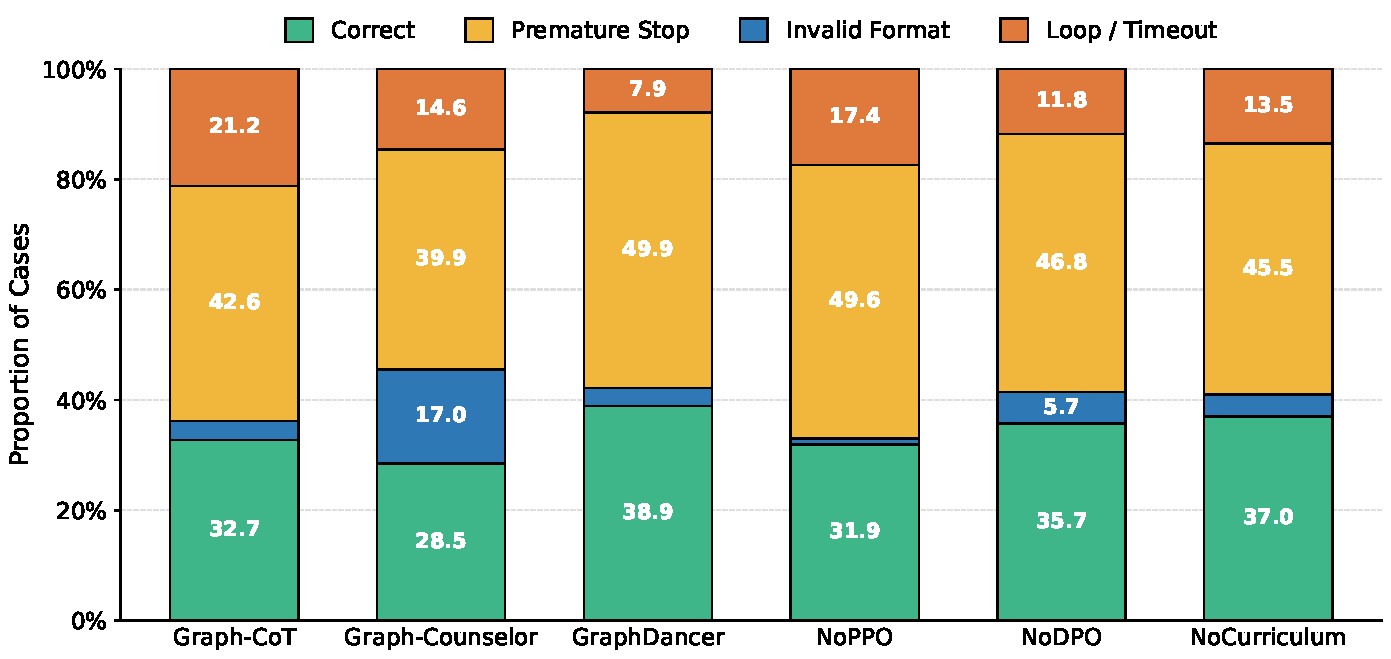
\includegraphics[width=\linewidth]{figures/error_breakdown_refined.pdf}
\vspace{-1.5em}
\caption{Outcome breakdown pooled over 890 questions across the four unseen GRBench domains. Each bar decomposes episodes into \textit{Correct} and three failure modes: \textit{Invalid Format}, \textit{Loop / Timeout}, and \textit{Premature Stop}. All six methods use \texttt{Qwen2.5-3B-Instruct} as the LLM backbone.}
\label{fig:error_breakdown}
\vspace{-1em}
\end{figure}

% \smallskip
To further analyze why \ours performs better, we decompose each episode into four outcomes: \textit{Correct}, \textit{Invalid Format} (invalid tool calls), \textit{Loop / Timeout} (exceeding the interaction budget), and \textit{Premature Stop} (terminating with an incorrect answer). Figure~\ref{fig:error_breakdown} reports the distribution for Graph-CoT and Graph-Counselor (both with the \texttt{Qwen2.5-3B-Instruct} backbone, the same as \ours), full \ours, and three ablation versions.

PPO drives most of the \textit{Loop / Timeout} reduction: NoPPO retains $17.4\%$ Loop / Timeout against Graph-CoT's $21.2\%$ and \ours's $7.9\%$, and its \textit{Correct} rate ($31.9\%$) falls below Graph-CoT. DPO instead targets schema adherence: NoDPO nearly doubles \textit{Invalid Format} ($3.3\% \to 5.7\%$) while leaving \textit{Loop / Timeout} close to the full system. The curriculum sits between the two: NoCurriculum compresses Loop / Timeout only to $13.5\%$ and trails the full system by $1.9$ points on \textit{Correct}, indicating that the easy-to-hard schedule mainly helps the agent learn when to terminate.
In other words, PPO produces the navigation behavior that suppresses Loop / Timeout, DPO produces the format compliance that suppresses Invalid Format, and the graph-aware curriculum amplifies both. Residual errors in the full system concentrate on \textit{Premature Stop} ($49.9\%$), where the agent fails decisively rather than wandering. Per-domain behavioral diagnostics (VF, VC, EH) are reported in Appendix~\ref{sec:appendix_behavior}.

% First, \ours substantially reduces navigational paralysis. The base model (\texttt{Qwen2.5-3B-Instruct}) and Vanilla PPO frequently encounter \textit{Loop / Timeout} errors (33.4\% and 31.5\%, respectively), suggesting that the agents often get ``lost'' in the graph, repeating actions or wandering without a clear stopping criterion. \ours nearly halves this rate to \textbf{19.3\%}, demonstrating that the curriculum effectively teaches the agent to navigate purposefully and recognize when to terminate a search.

% Second, errors shift toward decisiveness. The reduction in loops is accompanied by a dominant rise in \textit{Premature Stop} errors (71.3\%). While still an error, this represents a qualitative improvement: the agent is no longer stalling or crashing, but actively attempting to formulate an answer. This ``decisive but hasty'' behavior indicates that the model has internalized the \textit{mechanics} of retrieval, though it occasionally underestimates the depth of reasoning required for complex queries, which is preferable to aimless wandering.

% Third, \ours demonstrates improved stability over Vanilla PPO. Standard RL fine-tuning often degrades instruction-following capabilities, as reflected in Vanilla PPO’s spike in \textit{Format Error} errors (12.9\%). \ours mitigates this instability (9.3\%), maintaining stronger adherence to function-calling schemas despite the challenges of exploration.

\subsection{Evidence-Grounded Accuracy}
\label{sec:eh}

Rouge-L and GPT4Score reward accurate final answers but cannot tell whether the model actually retrieved supporting evidence or guessed. We complement them with an evidence-grounded view  in Table~\ref{tab:eh}. Each episode is decomposed by exact-match correctness (EM) and evidence hit (EH; whether the model's tool observations contain the gold answer). $\mathrm{P}(\text{EM} \mid \text{EH})$ then measures evidence-to-answer conversion, and $\mathrm{P}(\text{EM} \mid \neg\text{EH})$ characterizes the probability that the model guesses correctly without retrieving good evidence.

\begin{table}[t]
\centering
\small
\setlength{\tabcolsep}{2.8pt}
\scalebox{0.85}{
\begin{tabular}{lcccc}
\toprule
Method & EH$\uparrow$ & P(EM$\mid$EH)$\uparrow$ & P(EM$\mid\neg$EH) & EM$\uparrow$ \\
\midrule
Graph-CoT        & 40.5 & 69.8 & 7.4 & 32.7 \\
Graph-Counselor  & 39.0 & 73.2 & 0.0 & 28.5 \\
\textbf{\ours}   & \textbf{43.8} & \textbf{77.4} & 8.8 & \textbf{38.9} \\
\bottomrule
\end{tabular}
}
\caption{Evidence-grounded accuracy (\%) pooled over 890 questions across the four unseen GRBench domains. EH is the fraction of episodes that surface answer-supporting evidence in tool observations; $\mathrm{P}(\text{EM}\mid\text{EH})$ and $\mathrm{P}(\text{EM}\mid\neg\text{EH})$ condition exact-match accuracy on the presence or absence of retrieved evidence. All methods use \texttt{Qwen2.5-3B-Instruct} as the LLM backbone.}
\vspace{-1em}
\label{tab:eh}
\end{table}

Consistent with intuition, evidence hit is the dominant driver of correctness: $\mathrm{P}(\text{EM}\mid\text{EH})$ is roughly an order of magnitude above $\mathrm{P}(\text{EM}\mid\neg\text{EH})$ in every row, and Graph-Counselor is the limiting case at $\mathrm{P}(\text{EM}\mid\neg\text{EH}) = 0$ (it never returns a correct answer without first retrieving the gold entity). Among compared methods, \ours achieves the highest EH ($43.8\%$) and the highest evidence-conversion rate ($77.4\%$), indicating that DPO post-training improves both retrieval coverage and the conversion of retrieved evidence into a correct answer.
Graph-Counselor's clean grounding behavior is offset by its lower EH, capping its EM at $28.5\%$.

\subsection{Case Study}
\label{sec:case_study}

We analyze a Medium-difficulty instance from the unseen \textsc{E-commerce} domain to inspect whether \ours learns transferable graph exploration behavior. The question asks for the price of an item \textit{bought together} with a specific loudspeaker, requiring the two-hop path \textit{Anchor Item} $\rightarrow$ \textit{Neighbor Item} $\rightarrow$ \textit{Price}.

Figure~\ref{fig:case_study} compares two trajectories. Both models find the anchor node (\texttt{B000NJIYHY}), but Graph-CoT (with the \texttt{Qwen2.5-3B-Instruct} backbone, the same as \ours) fails at the expansion step: it checks that a \textit{bought together} neighbor exists with \texttt{NodeDegree}, then invents a neighbor ID instead of retrieving it, causing an invalid function call. It subsequently queries the anchor item's price and returns the wrong answer.

\ours instead follows the required graph protocol: it retrieves the neighbor ID with \texttt{NeighborCheck}, then queries that node's price with \texttt{NodeFeature}, yielding the correct answer (\$12.95). This illustrates a transferable exploration pattern: first obtain the relevant node ID, then query its attributes.

\begin{figure}[t]
\centering
\begin{tcolorbox}[
    colback=teal!10!white,
    colframe=teal!40!white,
    title=,
    fonttitle=\small,
    coltitle=black,
    boxsep=0.75mm,
    left=1.5mm,
    right=1.5mm,
    top=1mm,
    bottom=1mm
    ]
    \scriptsize
    % --- Part 1: Question ---
    \textbf{Question (\textsc{E-Commerce})}: \\
    {\ttfamily What is the usual price of the items often purchased together with ``PYLE-PRO PPHP1293 - 800 Watt 12'' Two-Way Plastic Molded Loudspeaker''?} \\
    \rule{\linewidth}{0.5pt} \\
    % --- Part 2: Baseline ---
    \textbf{Graph-CoT} (\texttt{Qwen2.5-3B-Instruct}): \\
    {\ttfamily
    <think> Locate the item node first. </think> \par
    <graph> RetrieveNode[PYLE-PRO...] </graph> \par
    <information> [B000NJIYHY] </information> \par
    <think> Check degree of bought\_together neighbors. </think> \par
    <graph> NodeDegree[B000NJIYHY, bought\_together] </graph> \par
    <information> [1] </information> \par
    {\color{myred} <think> Access the neighbor using index 0. </think>} \par
    {\color{myred} <graph> NodeFeature[B000NJIYHY\_bought\_together\_\\\_item\_0, price] </graph>} \par
    {\color{myred} <information> Node or feature name does not exist. </information>} \par
    <think> Access failed. I will assume the price is similar to the original item. </think> \par
    <graph> NodeFeature[B000NJIYHY, price] $\rightarrow$ [140.43] </graph> \par
    <answer> 140.43 </answer> \quad {\color{myred} \textbf{(\ding{55} Wrong: Returns anchor price)}}
    } \\
    \rule{\linewidth}{0.5pt} \
    % --- Part 3: Ours ---
    \textbf{\ours} \\
    {\ttfamily
    <think> Find anchor node, then find its neighbors. </think> \par
    <graph> RetrieveNode[PYLE-PRO...]</graph> \par
    <information> [B000NJIYHY] </information> \par
    <think> I need the ID of the neighbor to query its price. </think> \par
    {\color{teal} \textbf{<graph> NeighborCheck[B000NJIYHY, bought\_together] </graph>}} \par
    <information> ['B000E1U4WY'] </information> \par
    <think> Now query the price of the found neighbor B000E1U4WY. </think> \par
    {\color{teal} \textbf{<graph> NodeFeature[B000E1U4WY, price] </graph>}} \par
    <information> [12.95]</information> \par
    <answer> 12.95 </answer> \quad {\color{mygreen} \textbf{(\ding{51} Correct)}}
    }
\end{tcolorbox}
\vspace{-0.5em}
\caption{Case study. Graph-CoT finds the anchor item but invents a neighbor ID and returns the anchor price, while \ours explicitly retrieves the neighbor through \texttt{NeighborCheck} before querying its price.}
\label{fig:case_study}
\vspace{-1.5em}
\end{figure}

\section{Related Work}
\noindent \textbf{LLM Agents on Graphs.}
Early work integrates LLMs with graphs through feature extraction for graph neural networks \citep{santoro2017simple,zhao2023learning,jin2023heterformer,duan2024simteg} or single-pass retrieval over textualized graph context \citep{gao2023retrieval,ye2024language}.
These methods are effective for exposing graph-derived information to LLMs, but they do not explicitly train models to conduct multi-round graph exploration.
Recent prompting-based graph agents address this by interleaving reasoning with graph actions \citep{luo2024reasoning,wang2024knowledge}: Graph-CoT \citep{jin2024graph} traverses external graphs through iterative function calls, Graph-Counselor \citep{gao2025graph} uses a multi-agent prompting framework, and GraphRunner \citep{kashmira2025graphrunner} separates planning, verification, and execution to reduce traversal errors.
Another line introduces RL into graph agents, including Graph-MCTS \citep{liu2025graphmcts}, Graph-o1 \citep{liu2025grapho1}, GraphScout \citep{ying2026graphscout}, Graph-R1 \citep{luo2025graph}, and Structure-R1 \citep{wu2025structure}.
These methods improve inference-time search or post-training, but typically do not couple online executable rewards and offline trajectory preferences under the same structural curriculum.
\ours differs by using a unified post-training pipeline in which PPO, DPO, and a graph-aware curriculum jointly internalize transferable graph exploration behavior.

\smallskip
\noindent \textbf{LLM Post-Training and Curriculum Learning.}
Preference optimization \citep{schulman2017proximal,rafailov2023direct,shao2024deepseekmath,yu2026dapo} has become central to LLM post-training \citep{ouyang2022training,guo2025deepseek}, while curriculum learning \citep{bengio2009curriculum} improves long-horizon training through easy-to-hard scheduling \citep{parashar2025curriculum}, adaptive rollout control \citep{shen2025thinking}, and multi-objective balancing \citep{hammoud2025train}.
Most existing applications focus on math, code, or unstructured web search \citep{jin2025search}. We instead combine PPO, DPO, and curriculum learning in structured graph environments mediated by typed function calls.

\section{Conclusion}
We present \ours, a two-stage post-training framework for graph reasoning with LLMs.
PPO teaches executable graph interaction under rule-based rewards, DPO refines the policy with self-generated preferences, and a graph-aware curriculum organizes both stages by information-seeking complexity.
Training only on \textsc{Academic}, \ours generalizes to four unseen domains and OOD question types with a 3B backbone.
The results suggest that transferable graph exploration requires training signals matched to graph interaction structure, beyond stronger prompting or larger backbones.

\end{spacing}

\section*{Limitations}
\label{sec:limitations}
Our framework involves several design choices, including the curriculum shape, biased-mixture schedule, PPO hyperparameters, and DPO preference-pair construction. Due to the high computational cost of two-stage post-training, we do not perform an exhaustive sensitivity study over this space, such as varying mixture coefficients, level priors, KL strength, or rollout budgets. Pilot runs indicate that auxiliary format rewards, biased-mixture sampling, and preference-pair quality can substantially affect training stability and final performance, but a systematic ablation with complete learning curves is left to future work.

Additionally, we adopt the deterministic Graph-CoT tool API and the GRBench benchmark, both of which provide clean, well-typed function signatures and exact retrieval. Real knowledge graphs do not look like this: schemas change between snapshots, entity mentions are ambiguous, coverage is uneven, and tool calls go through a learned retriever rather than a deterministic lookup. We leave the transfer of our policy to such settings as an open question for future work. Our evaluation also focuses on factual question answering over the four GRBench unseen domains, which exercise multi-hop traversal and aggregation but do not stress open-ended generation, long-horizon planning beyond the $T_{\max}{=}10$ budget, or interactive multi-turn dialogue.

\section*{Ethical Considerations}
Our work enhances an LLM's ability to explore graph-structured knowledge through executable function calls, which can improve grounding and factuality but also introduces risks when connected to real-world graphs. In particular, graph tool APIs may expose sensitive information, such as proprietary relations or user data, and could be misused for broad traversal or data exfiltration if access is not carefully controlled. Deployments should therefore enforce strict authentication and authorization, least-privilege function permissions, auditing, and redaction of sensitive fields in tool outputs. Because node attributes and observations may contain untrusted text, systems are also vulnerable to prompt-injection attacks that attempt to manipulate subsequent actions. Tool outputs should be sanitized and isolated, and all calls should be validated against an allowlist of functions and argument schemas. Finally, while our PPO+DPO post-training pipeline reduces some behavioral failures, such as invalid calls, it does not guarantee correctness. Agents may still retrieve incomplete evidence, prefer a flawed trajectory, or terminate prematurely. We therefore view it as decision support rather than a substitute for expert judgment, especially in high-stakes domains. We also use an existing public benchmark (GRBench) and do not collect any new user data. We inspected the released graphs for sensitive personal information and did not find private identifiers (e.g., emails, phone numbers, addresses); person names that appear (e.g., academic authors) are part of publicly available entity records. The benchmark is not sourced from user-generated content, and we did not observe offensive/toxic text; we do not release any additional personal information beyond the benchmark.

\bibliography{custom}

\newpage
\appendix
\section{More Experimental Details}
\subsection{Baselines Details}
\label{app:baselines}
\begin{itemize}[leftmargin=*]
\item \textbf{TextRAG} \cite{gao2023retrieval} treats graph-associated textual fields as an unstructured corpus.
For each question, it retrieves relevant text units and appends them to the prompt before a single answer-generation step.
It does not expose typed graph relations or executable graph functions to the LLM.

\item \textbf{GraphRAG} \cite{ye2024language} augments retrieved text with graph context by collecting and linearizing the local subgraph associated with the retrieved entry.
The resulting context is still consumed in a single forward pass, so the model cannot adaptively issue follow-up graph actions based on intermediate observations.

\item \textbf{Graph-CoT} \cite{jin2024graph} performs iterative graph reasoning through a reasoning-interaction-execution loop.
At each step, the LLM reasons about what information is needed, emits graph interactions such as node retrieval or neighbor checking, and then conditions on the executor's returned observations before deciding the next step.
We keep the original system instructions and few-shot examples from \citet{jin2024graph}.

\item \textbf{Graph-Counselor} \cite{gao2025graph} decomposes graph reasoning across multiple prompted agents.
It coordinates planning, thought, and execution agents to gather textual, structural, and degree information, and it performs backward checking to improve semantic consistency.
We use the released implementation with its default settings, including \texttt{max\_steps} = 10, \texttt{max\_reflect} = 2, and sampling temperature $0.7$.

\item \textbf{Graph-MCTS} \cite{liu2025graphmcts} uses Monte Carlo Tree Search to guide graph exploration.
The search procedure evaluates alternative graph traversal actions through selection, expansion, simulation, and backpropagation, helping the LLM choose more promising graph paths than a purely greedy prompting strategy.

\item \textbf{Graph-o1} \cite{liu2025grapho1} extends MCTS-style graph exploration with an agent-environment formulation and reward-driven optimization over text-attributed graphs.
It selectively explores and retrieves relevant subgraph elements through multi-turn interaction, rather than encoding a large retrieved subgraph as static context.
\end{itemize}

\subsection{Hyperparameters}
\label{app:hyperparameters}

\noindent \textbf{Graph Executor and Interaction Budget.}
All models interact with the same graph executor and function API.
We set \texttt{max\_turns} = 10. Within each turn, the model may emit a batch of graph calls inside a \texttt{<graph>} block, which are executed deterministically.
Table~\ref{tab:prompt_template} shows the full prompt template used for all rollouts.

\smallskip
\noindent \textbf{PPO Training.}
We use the same decoding configuration for inference-time generation and PPO rollout generation: temperature $0.7$, top-$p$ $0.8$, and top-$k$ $20$.
We perform PPO for $200$ steps with a global rollout buffer and minibatch size $128$ (microbatch size $8$ per GPU).
The KL penalty coefficient is fixed to $\gamma=0.001$ relative to the reference policy.
We use policy clip ratio $0.2$ and value clip range $0.5$.
The actor and critic learning rates are $10^{-6}$ and $10^{-5}$, respectively.
For the reward in Eq.~\ref{eq:reward}, we set $\lambda_{\text{struct}} = 0.2$ and $\lambda_{\text{final}} = 0.1$.

\smallskip
\noindent \textbf{DPO Training.}
We sample $M=8$ trajectories per \textsc{Academic} training question from the PPO checkpoint, using temperature $1.0$, top-$p$ $0.95$, and the same $T_{\max}=10$ interaction budget.
We perform DPO with $\beta=0.1$, learning rate $2\times10^{-7}$, linear warmup over the first $5\%$ of steps, and linear decay.
Training runs for $100$ optimization steps with global batch size $64$ ($8$ GPUs $\times$ per-device batch size $2$ $\times$ gradient accumulation $4$).
We use AdamW in \texttt{bf16}, gradient checkpointing, and FSDP full-shard with parameter and optimizer offload.

\smallskip
\noindent \textbf{Curriculum Configuration.}
For both PPO and DPO, we use the Gaussian curriculum scheduler with shape parameter $\kappa=3$ and $\sigma=0.75$.
The time-varying mixture in Eq.~\ref{eq:mixture_sampler} uses $\eta_{\text{start}}=0.2$ and $\eta_{\text{end}}=0.8$.
The fixed level-bias prior is $q=[0.5,0.5,0]$ over \{Easy, Medium, Hard\}.

% Optional GRPO did-not-converge writeup, currently commented out via
% \iffalse / \fi. Restore by removing the guards if a reviewer asks
% for an explicit GRPO comparison.
\iffalse
\subsection{GRPO Attempt}
\label{app:grpo}
We initially considered substituting GRPO \cite{guo2025deepseek} for PPO in the RL stage, motivated by recent reports of GRPO outperforming PPO on math and reasoning benchmarks. With the paper recipe (group size 8, no critic, KL coefficient $0.001$) on the same \texttt{Qwen2.5-3B-Instruct} backbone and \textsc{Academic} training set, the policy did not converge: format-validity rate collapsed early in training, and exact-match reward did not exceed the base-model floor over the same $200$-step horizon used for PPO. Whether GRPO can be made to work in this multi-turn graph-interaction setting is an open question; for this paper we report the PPO-based pipeline.
\fi

\section{More Analysis}
\label{sec:appendix_analysis}

\subsection{Difficulty-wise Breakdown of Cross-Domain Gains}
\label{sec:curriculum_analysis}

Table~\ref{tab:difficulty_breakdown} breaks down Rouge-L by structural difficulty (Section~\ref{sec:round_types}), contrasting \ours against Graph-CoT and Graph-Counselor on the four unseen GRBench domains.

\begin{table}[t]
\centering
\small
\setlength{\tabcolsep}{4pt}
\scalebox{0.84}{
\begin{tabular}{llcccc}
\toprule
Domain & Method & Easy & Medium & Hard & OOD \\
\midrule
\multirow{3}{*}{\textsc{E-commerce}} & Graph-CoT & 82.34 & 38.47 & 11.64 & 3.49 \\
 & Graph-Counselor & 77.73 & 40.76 & 9.11 & \textbf{4.64} \\
 & \textbf{\ours} & \textbf{87.86} & \textbf{54.31} & \textbf{16.33} & 2.85 \\
\midrule
\multirow{3}{*}{\textsc{Literature}} & Graph-CoT & 63.52 & 55.14 & 6.59 & 1.67 \\
 & Graph-Counselor & 61.97 & 52.38 & 6.48 & 3.45 \\
 & \textbf{\ours} & \textbf{73.52} & \textbf{58.26} & \textbf{6.68} & \textbf{6.50} \\
\midrule
\multirow{3}{*}{\textsc{Healthcare}} & Graph-CoT & 63.23 & 7.09 & 0.00 & -- \\
 & Graph-Counselor & 63.12 & 11.45 & \textbf{5.00} & -- \\
 & \textbf{\ours} & \textbf{66.51} & \textbf{15.17} & 0.00 & -- \\
\midrule
\multirow{3}{*}{\textsc{Legal}} & Graph-CoT & 52.93 & 9.04 & 4.39 & 4.29 \\
 & Graph-Counselor & 26.26 & 0.00 & 0.00 & 3.92 \\
 & \textbf{\ours} & \textbf{60.85} & \textbf{30.91} & \textbf{21.66} & \textbf{28.67} \\
\bottomrule
\end{tabular}
}
\caption{Difficulty-wise Rouge-L (\%) on the four unseen GRBench domains. ``--'' marks splits with no test samples (see Table~\ref{tab:data_stats}); the only such split is \textsc{Healthcare} OOD. All three methods use \texttt{Qwen2.5-3B-Instruct} as the LLM backbone.}
\vspace{-0.5em}
\label{tab:difficulty_breakdown}
\end{table}

\ours wins Easy and Medium across all four domains. The largest absolute gains over Graph-CoT concentrate on \textsc{Legal}, where Easy improves $+7.92$, Medium $+21.87$, Hard $+17.27$, and OOD $+24.38$. \textsc{Literature} Medium also moves substantially ($+3.12$ over Graph-CoT). The two cells where Graph-Counselor outperforms \ours are both at the corners of the benchmark: \textsc{Healthcare} Hard ($5.00$ vs.\ $0.00$), a 20-question bucket of extreme-aggregation queries, and \textsc{E-commerce} OOD ($4.64$ vs.\ $2.85$). Graph-Counselor itself collapses on \textsc{Legal} (Easy $26.26$, Medium $0.00$), reflecting the volatility of multi-agent prompting at the 3B scale.

\subsection{Behavioral Analysis of Graph Interaction}
\label{sec:appendix_behavior}

Outcome metrics alone do not reveal whether a model has internalized the multi-round \texttt{reasoning$\rightarrow$action$\rightarrow$observation} procedure. We therefore complement Table~\ref{tab:main} with behavioral diagnostics computed from execution traces, comparing \ours against Graph-CoT and Graph-Counselor (both on \texttt{Qwen2.5-3B-Instruct}).

We report the following metrics: (1) Valid Format (\textsc{VF}), the proportion of trajectories that follow the required \texttt{<think>} / \texttt{<graph>} / \texttt{<information>} / \texttt{<answer>} structure; (2) Valid Call (\textsc{VC}), the fraction of tool calls that pass schema validation; and (3) Evidence Hit (\textsc{EH}), the fraction of episodes where the normalized gold answer appears in any returned tool observation. Graph-Counselor uses a free-form Plan / Thought / Action / Observation protocol that does not map onto the \texttt{<think>/<graph>} block structure, so \textsc{VF} and \textsc{VC} are not applicable; \textsc{EH} is well-defined regardless of protocol since it inspects retrieved observations rather than format compliance.

Table~\ref{tab:behavior_diag} shows that \ours substantially improves \textsc{VF} over Graph-CoT across all domains (e.g., 31.9 $\to$ 46.7 on \textsc{Healthcare}, 42.8 $\to$ 54.4 on \textsc{Legal}), confirming that curriculum-based post-training strengthens adherence to the multi-round interaction protocol. In terms of EH, the three methods cluster within $\sim$3 points on \textsc{E-commerce} and \textsc{Literature}; Graph-Counselor wins \textsc{Healthcare} \textsc{EH} ($31.11$ vs.\ $21.9$ for \ours) but collapses on \textsc{Legal} ($17.78$ vs.\ $43.9$), reflecting the volatility of multi-agent prompting at the 3B scale.

\begin{table}[t]
\centering
\small
\setlength{\tabcolsep}{4.6pt}
\scalebox{0.85}{
\begin{tabular}{llccc}
\toprule
Domain & Model & VF $\uparrow$ & VC $\uparrow$ & EH $\uparrow$ \\
\midrule
\multirow{3}{*}{\textsc{E-commerce}}
& Graph-CoT       & 62.5 & 99.1 & 49.0 \\
& Graph-Counselor & -- & -- & 49.5 \\
& \textbf{\ours}  & \textbf{78.0} & 99.1 & \textbf{50.0} \\
\midrule
\multirow{3}{*}{\textsc{Literature}}
& Graph-CoT       & 48.8 & 98.6 & 51.7 \\
& Graph-Counselor & -- & -- & 55.0 \\
& \textbf{\ours}  & \textbf{70.0} & \textbf{100.0} & \textbf{55.8} \\
\midrule
\multirow{3}{*}{\textsc{Healthcare}}
& Graph-CoT       & 31.9 & \textbf{99.3} & 20.4 \\
& Graph-Counselor & -- & -- & \textbf{31.1} \\
& \textbf{\ours}  & \textbf{46.7} & 98.9 & 21.9 \\
\midrule
\multirow{3}{*}{\textsc{Legal}}
& Graph-CoT       & 42.8 & \textbf{97.8} & \textbf{46.7} \\
& Graph-Counselor & -- & -- & 17.8 \\
& \textbf{\ours}  & \textbf{54.4} & 89.1 & 43.9 \\
\bottomrule
\end{tabular}
}
\caption{Behavioral analysis of execution traces on the four unseen GRBench domains. \textsc{VF}: fraction of episodes following the required interaction format; \textsc{VC}: fraction of tool calls passing schema validation; \textsc{EH}: fraction of episodes where the normalized gold answer appears in any returned tool observation. All methods use \texttt{Qwen2.5-3B-Instruct} as the LLM backbone. Graph-Counselor's multi-agent Plan / Thought / Action / Observation protocol does not match the \texttt{<think>/<graph>} format definition of \textsc{VF}/\textsc{VC}; \textsc{EH} is computed from the concatenation of every observation returned to the agents.}
\label{tab:behavior_diag}
% \vspace{-0.5em}
\end{table}

\subsection{Question-Type Breakdown on \textsc{Literature}}
\label{sec:lit_qtype}

To localize the gains of \ours on \textsc{Literature}, we group test questions into four categories using a regex matcher over the canonical question templates from \citet{jin2024graph}. Table~\ref{tab:lit_qtype} reports exact match (EM) and Rouge-L for each category.

\begin{table}[t]
\centering
\small
\setlength{\tabcolsep}{2.2pt}
\scalebox{0.78}{
\begin{tabular}{lcccc}
\toprule
& Simple Lookup & Aggregation & Multi-hop & Set Ops. \\
& {\scriptsize $n{=}37$} & {\scriptsize $n{=}29$} & {\scriptsize $n{=}21$} & {\scriptsize $n{=}5$} \\
\cmidrule(lr){2-2} \cmidrule(lr){3-3} \cmidrule(lr){4-4} \cmidrule(lr){5-5}
& EM$\uparrow$\,/\,R-L$\uparrow$ & EM$\uparrow$\,/\,R-L$\uparrow$ & EM$\uparrow$\,/\,R-L$\uparrow$ & EM$\uparrow$\,/\,R-L$\uparrow$ \\
\midrule
Graph-CoT        & 43.24\,/\,49.34 & 55.17\,/\,55.17 & 28.57\,/\,32.02 & 20.00\,/\,40.45 \\
Graph-Counselor  & 48.65\,/\,55.87 & 48.28\,/\,48.28 & 28.57\,/\,29.32 & 0.00\,/\,16.26 \\
\textbf{\ours}   & \textbf{51.35}\,/\,\textbf{61.24} & \textbf{58.62}\,/\,\textbf{58.62} & \textbf{33.33}\,/\,\textbf{35.46} & \textbf{40.00}\,/\,\textbf{40.99} \\
\bottomrule
\end{tabular}
}
\caption{Question-type breakdown on Literature (\%). Categories are derived by regex-matching the canonical question templates from \citet{jin2024graph}. All methods use \texttt{Qwen2.5-3B-Instruct} as the LLM backbone. Set Ops.\ = Set Operations.}
\vspace{-0.5em}
\label{tab:lit_qtype}
\end{table}

\ours achieves the best performance in all four categories under both metrics. The largest gain appears on \textbf{Multi-hop} questions, where \ours reaches $33.33\%$ EM, compared with $28.57\%$ for both Graph-CoT and Graph-Counselor ($+4.76$). On \textbf{Set Operations}, \ours doubles Graph-CoT's EM from $20.00\%$ to $40.00\%$, while Graph-Counselor falls to $0.00\%$ on this small 5-question subset. For \textbf{Aggregation}, \ours improves over Graph-CoT by $+3.45$ EM and over Graph-Counselor by $+10.34$ EM. \textbf{Simple Lookup} is the closest category: \ours still edges Graph-Counselor by $2.70$ EM and Graph-CoT by $8.11$ EM, while Graph-Counselor's relatively strong $48.65\%$ suggests that multi-agent prompting is effective for single-step retrieval when no multi-hop chaining is required.

\begin{table*}[!htbp]
\centering
\small
\setlength{\tabcolsep}{6pt}
\renewcommand{\arraystretch}{1.08}
\begin{tabularx}{\textwidth}{lX}
\toprule
\textbf{Component} & \textbf{Content} \\
\midrule
Task instruction
& \texttt{\detokenize{Solve a question answering task by repeating bundled steps that contain reasoning (<think>...</think>) followed by exactly one graph interaction (<graph>...</graph>). After each <graph> call, the environment returns feedback inside <information>...</information>. You may take as many steps as necessary.}} \\ \\

Output protocol
& \texttt{\detokenize{- Intermediate step: <think>...</think>}}
\newline
\texttt{\detokenize{  <graph>Function[...]</graph>}}
\newline
\texttt{\detokenize{  (then environment returns <information>...</information>.)}}
\newline
\texttt{\detokenize{- Final step: <think>...</think><answer>...</answer>}}
\newline
\texttt{\detokenize{  (no more graph calls).}} \\ \\

Available functions
& \texttt{\detokenize{RetrieveNode[keyword]            # retrieves the related node from the graph according to the query}}
\newline
\texttt{\detokenize{NodeFeature[Node, feature]        # returns detailed attribute information of Node for the given "feature" key}}
\newline
\texttt{\detokenize{NodeDegree[Node, neighbor_type]   # returns the number of "neighbor_type" neighbors of Node}}
\newline
\texttt{\detokenize{NeighborCheck[Node, neighbor_type] # lists the "neighbor_type" neighbors of Node and returns them}} \\ \\

Format rules
& \texttt{\detokenize{1) You MUST conduct reasoning inside <think>...</think> before every graph call and after every <information> you receive.}}
\newline
\texttt{\detokenize{2) Inside <graph>...</graph>, issue EXACTLY ONE function per step. Do NOT include any other text in <graph>.}}
\newline
\texttt{\detokenize{3) Do NOT fabricate <information>; it is ONLY produced by the environment immediately after your <graph> step.}}
\newline
\texttt{\detokenize{4) Keep thoughts concise and ONLY inside <think>. Do NOT put a graph call inside <think>, and do NOT put thoughts inside <graph>.}}
\newline
\texttt{\detokenize{5) The final output MUST contain ONLY one <answer>...</answer> block with the requested node main features (e.g., names), not node IDs.}} \\ \\

In-context examples
& \texttt{\detokenize{Here are some examples:}}
\newline
\texttt{\detokenize{{examples}}}
\newline
\texttt{\detokenize{(END OF EXAMPLES)}} \\ \\

Graph schema
& \texttt{\detokenize{Definition of the graph:}}
\newline
\texttt{\detokenize{{graph_definition}}} \\ \\

Question
& \texttt{\detokenize{Question:}}
\newline
\texttt{\detokenize{{question}}} \\ \\

\bottomrule
\end{tabularx}
\caption{Prompt template used for all rollouts in \ours. Placeholders (\texttt{\{examples\}}, \texttt{\{graph\_definition\}}, \texttt{\{question\}}) are instantiated per example. We use the same graph definitions as in~\citet{jin2024graph}.}
\label{tab:prompt_template}
\vspace{-0.5em}
\end{table*}

\end{document}
